%# -*- coding: utf-8-unix -*-

\chapter{相关技术}
\label{chap:related}

\section{基于内容推荐}

基于内容的推荐系统的特点是根据物品内容与用户偏好的契合度为用户进行推荐。系统首先需要通过文档、描述说明等资料对用户历史记录中的物品进行分析,建立物品档案;并基于物品的特征为用户建立偏好档案。为了能够直观、简单地为用户提供推荐,物品档案与用户偏好档案通常具有相同结构的模型。基于内容推荐算法首先将用户偏好和物品进行匹配。根据匹配度,我们可以得知用户对该物品的偏好程度。在假定用户档案可以精确反应用户偏好的前提下,可以根据用户档案为用户进行信息甄别与筛选,对解决信息超载问题有极大的帮助。

\subsection{基于内容推荐系统架构}
基于内容的推荐系统需要对物品和用户档案使用合适的方法进行分析,还需要衡量用户偏好和物品相似度的策略。系统可以细分为三个关键组件,分别是内容分析、档案学习以及物品过滤。

在内容分析组件处理之前,物品通常是非结构化的。一般需要对物品进行预处理以提取结构相关信息。该组件的主要任务就是通过特征提取将物品从源信息空间迁移到目标空间,将物品的内容表示成适当的格式,以供在后两个组件中使用。第二个组件是档案学习,它对表示用户偏好的数据进行收集、归纳以建立用户档案。通常,可以通过统计学方法对数据进行收集,通过机器学习的方法对档案进行归纳,归纳的过程就是从用户偏好的物品和不喜欢的物品中,推导出用户的用户的兴趣模型。第三个组件是物品过滤,利用用户偏好档案与物品的相似度为用户推荐新物品。根据相似度衡量方式,计算结果包括离散型相似度以及连续型相似度。
将候选物品列表根据相似度进行排序,就可以得到推荐列表。

\begin{figure}
 \centering
 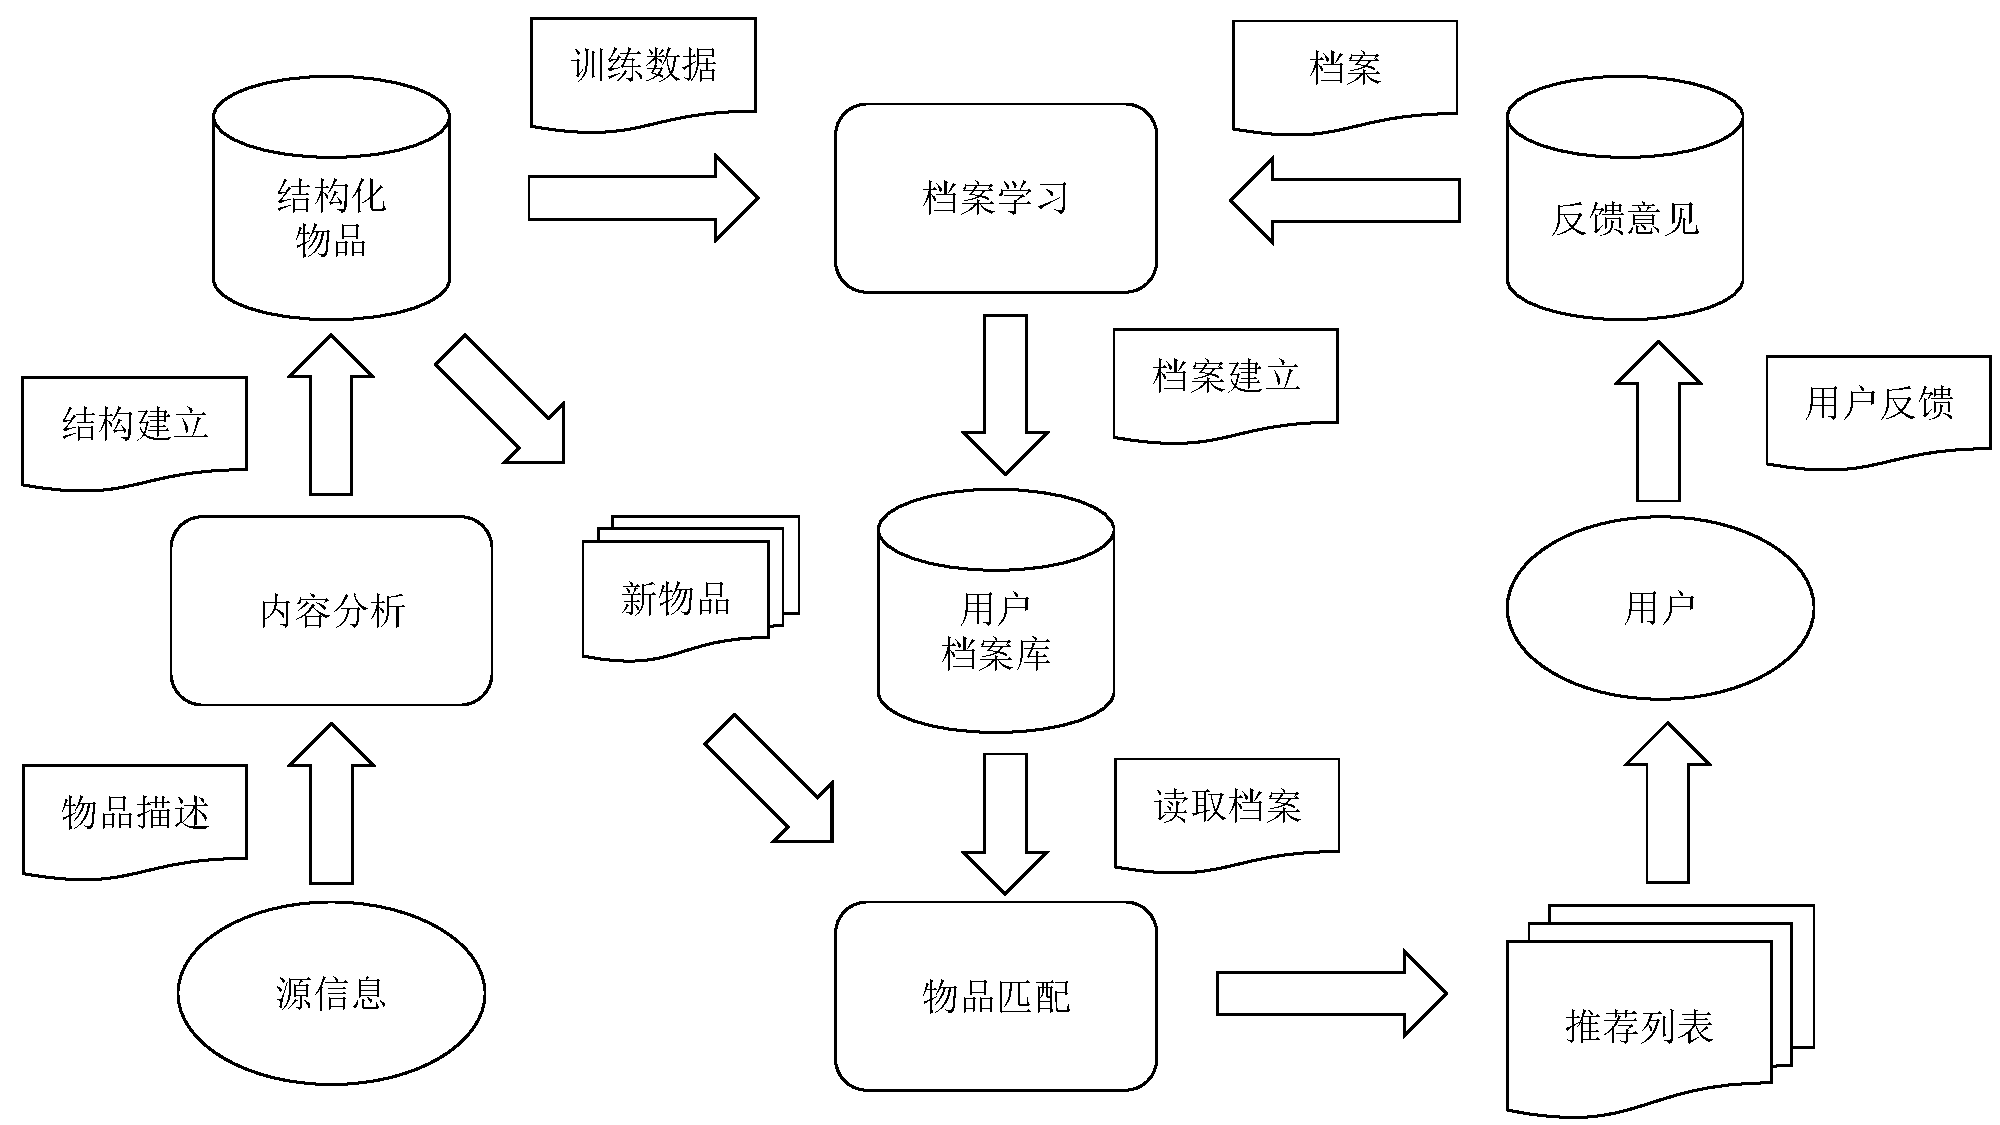
\includegraphics[width=0.75\linewidth]{02/1_cbr_arch.pdf}
 \bicaption[fig:cbr_arch]{推荐架构}{基于内容推荐算法的系统架构}{Fig}{Architecture of Content-based Recommender System}
\end{figure}

图\ref{fig:cbr_arch}展示了基于内容推荐算法的系统总体架构。其中椭圆形模块代表源数据,包括物品、用户信息;圆角矩形代表关键组件;圆柱形模块代表处理后的数据;箭头方向代表流程及数据流向。在内容分析组件中,通常会借用信息检索系统中的技术,为源信息中的物品提取特征,生成物品描述以及物品的结构化内容,并将其进行存储。

为了在档案学习阶段对用户档案进行创建及更新,需要存储用户对物品的评价反馈。用户反馈根据用户是否偏好该物品分为两种类型,分别是正反馈以及负反馈。根据反馈的获取方式,分为显式反馈和隐式反馈。其中,显式反馈由用户对物品的主动评价获得;而隐式反馈通过对用户行为的分析获得。显式反馈可以表明用户对物品的偏好程度以及相关性。总体上,显示反馈有三种表达方式。喜欢/反感 —— 用户使用二元评分机制将物品分为相关与不相关两类;打分 —— 使用离散的数值来表示对物品的评判。通常,将不同的喜好程度映射到不同的评分数值;文字评论 —— 依据用户对物品的评论来确定用户对物品的偏好。但需要自然语言处理的技术来判断评论属于正反馈还是负反馈。

为了向用户提供推荐物品,需要为用户$u_a$定义训练集$TR_a$,对于显式反馈而言,$TR_a$的形式可以是物品-评分集合。档案学习组件通过有监督学习的算法生成预测模型,即用户偏好档案;并将档案存储在档案仓库中,供物品过滤组件使用。对于每一个结构化的物品,物品过滤组件会预测用户是否对该物品有偏好。将用户最可能偏好的$K$个物品生成一份推荐列表展示给用户。此外,用户的偏好可能会随时间改变。因此,系统还需维护用户的实时信息,如用户对推荐列表中物品的评价等。根据新生成的训练集,使用档案学习组件对用户偏好进行自动更新。

\subsection{基于内容推荐系统的优点及缺点}

基于内容推荐系统的优点如下:

\begin{itemize}
 \item 用户独立性。基于内容推荐算法仅使用用户自己的评分记录建立其偏好档案。而基于协同过滤的方法需要其他用户的评分来为目标用户挑选出偏好最近邻的用户,也只能推荐近邻用户偏好的物品。
 \item 可解释性。可以为用户对推荐物品做出解释,例如列出物品的特征。这些特征也可以作为衡量推荐系统准确性的标准,便于对内容分析组件进行调整。在基于协同过滤的推荐算法中,唯一可以为用户进行解释就是另一个与目标用户偏好相似的用户也喜欢这个物品,缺乏可信度。
 \item 适用于物品冷启动。如果一项物品新加入到系统中,还没有被用户评分。基于协同过滤的推荐系统无法对此物品进行推荐。而基于内容的推荐系统可以克服物品冷启动问题。
\end{itemize}

同时,基于内容的推荐系统也有以下缺点:

\begin{itemize}
	\item 内容分析的局限性。基于内容推荐算法中的内容分析模块往往只能提取部分数量与类型的内容特征,这些特征作为建立用户偏好档案和物品推荐的主要依据。内容分析无法捕捉一些可能影响到用户购买决策的隐藏特征以及特征之间的关联。并且内容分析过程往往是领域相关的,通常需要丰富的专业领域知识。
	\item 过度匹配。基于内容推荐系统完全按照物品与用户偏好档案的匹配程度为物品进行打分、排序;并将排位较高的物品推荐给用户。因此,用户只能获取与其历史物品相似的推荐。推荐系统失去了新颖度。
	\item 用户冷启动问题。为了能够充分理解用户的偏好,建立有信服度的用户偏好档案。用户需要为一定数量的物品做出评价。因此,对于评价较少的新用户,系统难以给出可靠的推荐。
\end{itemize}

在机票推荐算法研究中,我们会在基于内容推荐的基础上,对物品内容分析及用户冷启动问题做出深入研究,以提升个性化机票推荐的效果。

\section{主题模型}


随着网络上的信息以及专业文献库越来越丰富,从文本中自动抽取有用的信息变得更加重要。这类模型在文档标标注、自动问答、自动文档摘要等应用场景起到很大作用。在信息检索、自然语言处理、机器学习等研究领域都对该类模型进行了深入研究。近年来,对有监督的文档自动分类研究得到了很多的关注。然而在很多情景下,既没有预先定义的标签库,也没有每篇文档的标签。文档库中的文档数量往往十分巨大,并且在诸如计算机、生物学等许多研究领域,文档的标签随着研究的进展发生很频繁的变化。对每篇文档进行人工标注也是不现实的。因而,基于无监督的文档模型具有更广阔的应用场景。

在研究实践中发现,基于生成模型的统计方法对解决这类问题很有帮助。这类模型统称为主题模型。主题模型使用无监督策略从文档库中为每篇文档抽取可解释的表示模型。该模型将每篇文档表示成主题的混合概率分布,每个主题包括一组共同出现频率较高的词。主题可以将具有相似含义的词语联系到一起,还能为包含多种含义的词语区分在使用情境下的具体意义。在先前的研究中,最常见的文档表示方法是词袋模型(bag of words)。这种模型将高维度的词汇向量转换到低维空间。综上,相比于其他的文档模型,主题模型有三点优势。第一,主题提取的过程是非监督的,即文档不需要标签以及初始化的步骤;第二,提取出的主题是可解释的,用户可以理解主题包含了哪些词汇;第三,每篇文档可以表示成多个主题的集合,可以捕捉主题之间的关系。


\subsection{主题模型概述}

主题模型的种类有很多。常见的方法包括潜在语义分析模型(LSA)、概率潜在语义分析模型(PLSA)以及潜在狄利克雷分布模型(LDA)等。

\subsubsection{LSA模型}
LSA的目的是为文档提取词汇的多重含义,并通过内容分析计算词汇以及文档之间的相似度。模型将文档库表示成一个矩阵,矩阵的每行代表一个词汇,每一列代表一篇文档。矩阵中每个元素代表该词汇出现在文档中获得频次。矩阵中的值需要进行加权处理,其考虑因素包括该词汇在文档中的重要程度以及该词汇在领域中总体信息丰富程度等。随后,对矩阵进行奇异值分解:(singular value decomposition, SVD)
\begin{equation}
	A = U\sum V^T
\end{equation}

原矩阵$A$的维度是$M \times N$,分别是文档库中文档的数量以及词库的数量。矩阵$U$的维度是$M \times K$,矩阵$\sum$的维度是$K \times K$,矩阵$V^T$的维度是$K \times N$。其中$\sum$是一个对角矩阵,对角线的值由矩阵$A$的特征值组成。一般情况下,不需要计算矩阵所有的特征值,只需最大的前$K$个值就可以有效覆盖原矩阵的信息。矩阵$U$中的每一列代表一个语义,每一行代表一篇文档。每个元素代表该文档与该语义的相关程度;矩阵$V$中的每一列代表一个关键词,每一行代表一个词汇。每个元素代表该词汇与该关键词的相关程度;而中间的矩阵$\sum$的元素则表示语义和关键词之间的相关性。LSA将原本的文档特征进行降维,减轻了词汇和语义之间的复杂对应关系。

\subsubsection{PLSA模型}
PLSA是Hofmann在1999年提出了模型。该模型属于基于统计的潜在类别模型,使用了基于概率的生成模型对LSA进行改进。该模型的主要目标是区分词汇在不同语境上下文中的不同含义,主要包括两个方面,首先针对一词多义的情况下进行词义消歧;然后根据对在相同上下文中出现的单词进行聚类以揭示主题的概念。PLSA模型在诸如计算机视觉、推荐系统等领域中得到应用。

PLSA包含$K$个语义层面的隐式变量,我们称之为主题。则模型的变量包含三类。分别是文档集合$d \in D = \{d_1, \dots, d_n\}$;词汇集合$w \in W = \{w_1, \dots, w_m\}$;主题集合$z \in Z = \{z_1, \dots, z_k\}$。其中,文档和词汇是已知变量,主题是未知变量,$K$代表主题的数量,通常由先验决定。

\begin{figure}
 \centering
 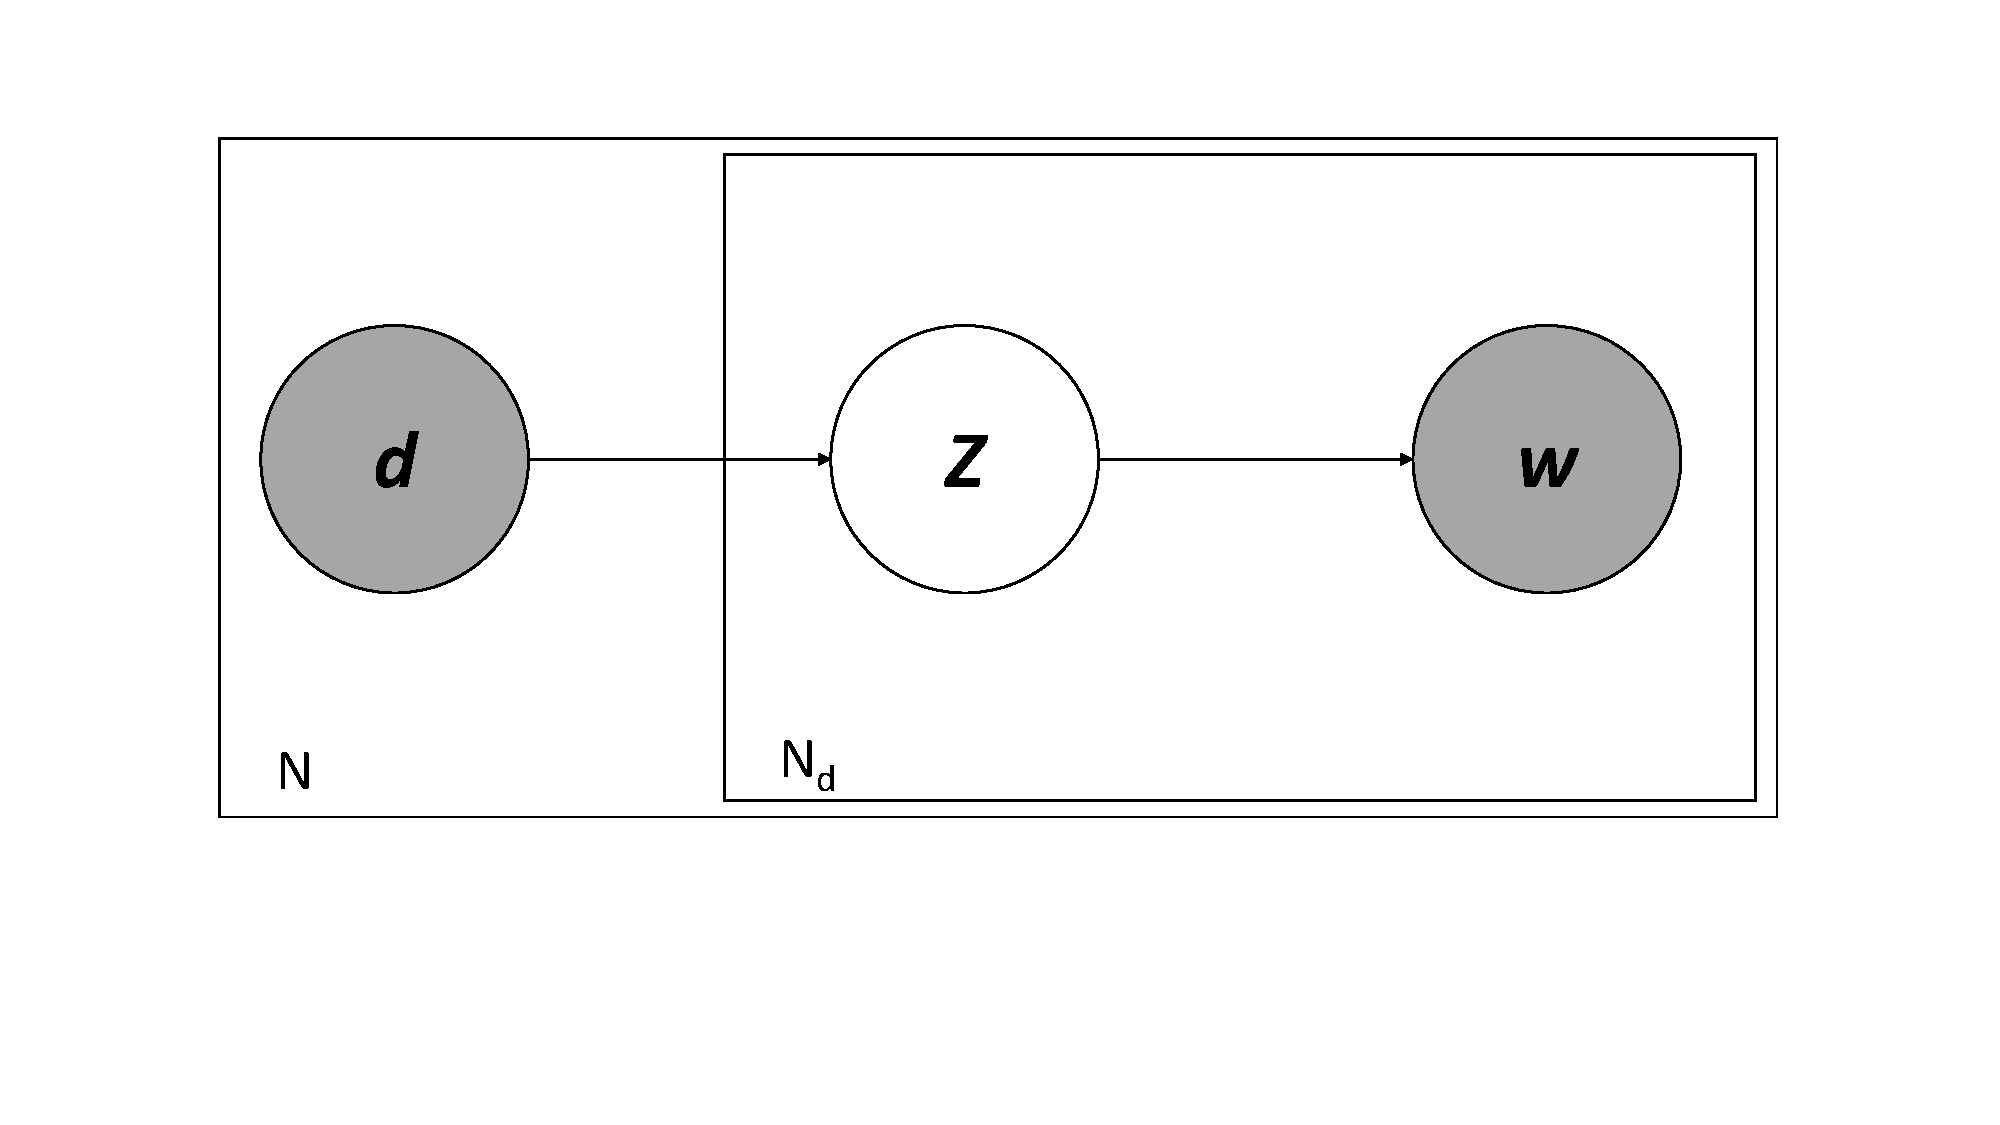
\includegraphics[width=0.7\linewidth]{02/2_plsa.pdf}
 \bicaption[fig:plsa]{PLSA}{PLSA概率图}{Fig}{Probability Graph for PLSA}
\end{figure}

图\ref{fig:plsa}是PLSA主题模型的概率图。$N$代指文档的数量,$N_w$代指每篇文档的词汇数量。带阴影的变量$d$,$w$分别代指文档与词汇,$z$代指隐式变量主题。每篇文档的生成过程描述如下:

\begin{enumerate}
\item 选择一篇文档 $d_n \sim P(d)$
\item 对于$d_n$中的每一个词汇
       \begin{enumerate}[fullwidth,itemindent=1em,label=(\alph*)]
       \item 基于多项式分布从文档中抽取一个主题,$z_i \sim P(z|d_n)$
       \item 基于多项式分布从主题中抽取一个词汇,$w_i \sim P(w|z_i)$
       \end{enumerate}
\end{enumerate}

一般情况下,我们可以认为对于给定的主题,词汇和文档是条件独立的,即$P(w|d,z) = P(w|z)$。则我们可以得到等式:
\begin{equation}
	P(w|d) = \sum_{z\in Z}P(w|z)P(z|d)
\end{equation}
\begin{equation}
	P(w,d) = \sum_{z\in Z}P(z)P(d|z)P(w|z)
\end{equation}

PLSA也可以应用在推荐系统中,将每位用户的历史购买记录视为一篇文档,购买过的没见物品视为一个词汇。可以根据模型分析出每篇文档与主题的关联。这里每个主题代表一种偏好习惯,根据每位用户的$P(z_k|d_i)$分布向量衡量用户间的相似度,就可以使用基于协同过滤的推荐算法。

\subsubsection{LDA模型}


在PLSA模型中,$P(z|d)$和$P(w|z)$都属于多项式分布,可以使用EM算法进行参数推导。但PLSA也有不足之处,首先参数$P(d)$是未知的,无法准确为一篇新文档设置概率值;其次,$P(z|d)$的数量随着文档的数量呈线性增长,可能会造成过拟合问题。

在LDA模型中,同样有文档-主题分布矩阵$\Theta$和主题-词汇分布矩阵$\Phi$两个待估参数,这两个参数分别服从超参数为$\alpha$和$\beta$的狄利克雷先验分布。LDA与PLSA的不同之处在于:PLSA中,两个参数$P(z|d)$和P(w|z)是固定的未知变量。计算这两个变量的过程是先按照文档-主题和主题-词汇概率分布生成文档,再使用极大似然估计算法(如EM算法)对两个参数进行估计。但LDA模型将文档-主题和主题-词汇的概率分布视作服从狄利克雷先验分布的变量,而不是固定的值。通过这样设定参数,可以使用与狄利克雷分布共轭的多项式分布进行参数推导,并且还可以克服过拟合问题,比PLSA具有更好的效果。

\begin{figure}
 \centering
 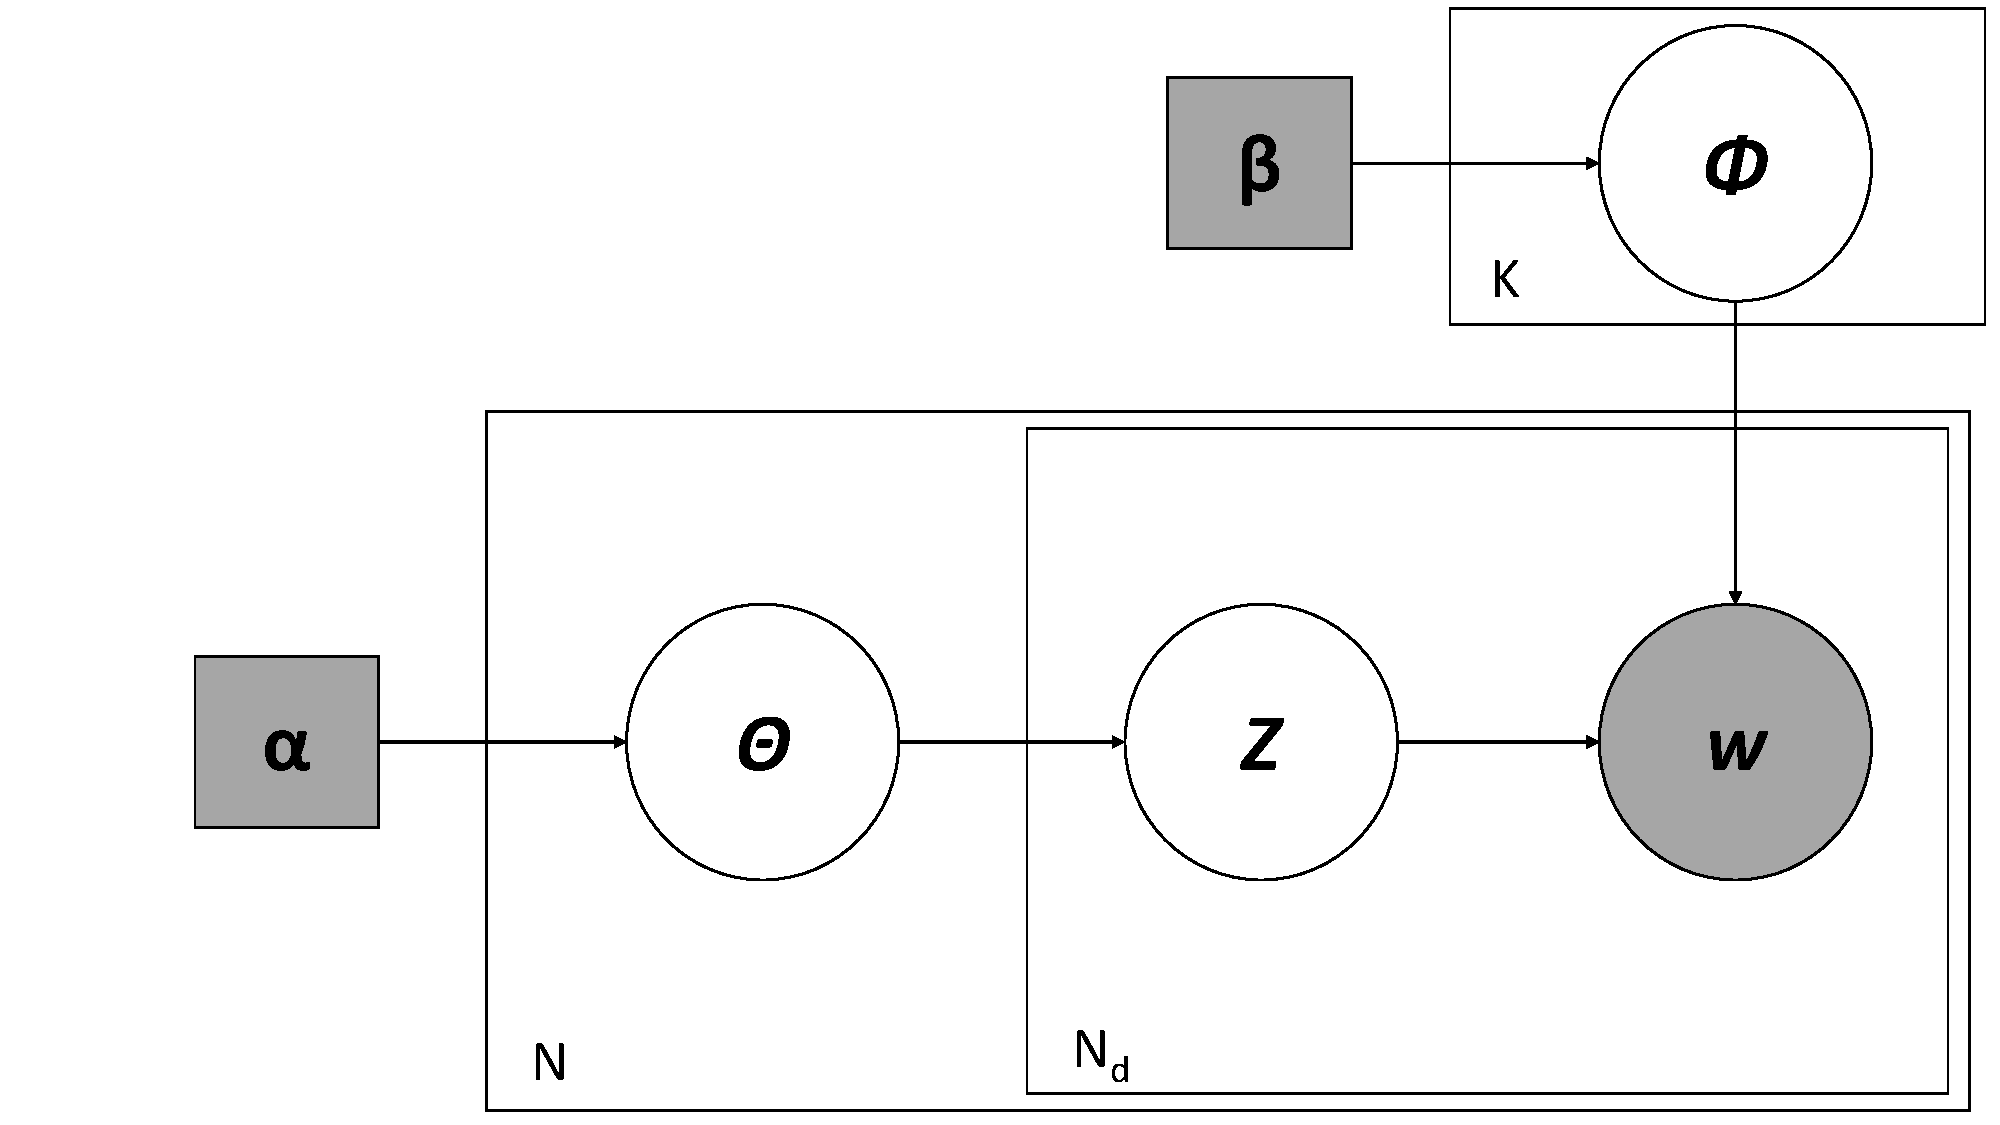
\includegraphics[width=0.7\linewidth]{02/3_lda.pdf}
 \bicaption[fig:lda]{LDA}{LDA概率图}{Fig}{Probability Graph for LDA}
\end{figure}

图\ref{fig:lda}是LDA主题模型的概率图。$N$代指文档的数量,$N_w$代指每篇文档的词汇数量,$K$代表主题的数量。带阴影的变量$\alpha$,$\beta$分别是两个待估参数的超参数,$w$代表词汇。每篇文档的生成过程描述如下:

\begin{enumerate}
\item 对每篇文档$d$,以狄利克雷先验初始化 $\theta_d \sim Dir(\alpha)$
\item 对每个主题$z$,以狄利克雷先验初始化 $\phi_z \sim Dir(\beta)$
\item 对于$d_n$中的每一个词汇
       \begin{enumerate}[fullwidth,itemindent=1em,label=(\alph*)]
       \item 基于多项式分布从文档中抽取一个主题,$z_i \sim Multi(\theta_{d_n})$
       \item 基于多项式分布从主题中抽取一个词汇,$w_i \sim Multi(\phi_{z_i})$
       \end{enumerate}
\end{enumerate}

LDA模型的参数具有超参数先验,如果先验足够准确,可以提升参数估计的准确率。并且适用于词汇数量较少的文档训练。此外,具有先验的参数可以对超参数进行调整,以适应不同的应用场景。在我们的研究中,使用主题模型来挖掘乘客和机票特征之间的关系,在共享账户情景中可以预测出乘客分布概率,以提升机票推荐的效果。

\section{模型参数估计}

在统计学中,参数估计代表使用样本数据来估计总体数据概率分布的过程。在机器学习模型中,参数往往用于描述模型的状态。而模型的真实分布是未知的,需要根据已知自变量和因变量之间的关系对整体模型的参数进行估计。一般使用独立同分布的数据集$\mathcal{X}$来表示随机变量$X$的一组观测值。$\theta$代指$X$的参数集合,取决于随机变量服从的分布。参数估计包括两个方面,第一类问题是估计参数$\theta$使得$\mathcal{X}$的出现概率最大;第二类问题是估计新的观测值$\tilde{x}$的概率。第一类问题是估计问题,而第二类问题是预测分类问题。

参数估计的方法有很多,本节我们主要介绍两种训练模型常用方法,分别是最大似然估计(Maximum Likelihood Estimation,MLE)以及最大后验概率(Maximum a Posteri,MAP)。

\subsection{最大似然估计}

最大似然估计的目标是估计参数使其最大化似然函数。通常似然函数都有如下的形式:
\begin{equation}
\label{eq:ml}
	L(\theta|\mathcal{X}) = p(\mathcal{X}|\theta) = \bigcap_{x \in \mathcal{X}}{X=x|\theta} = \prod_{x \in \mathcal{X}}p(x|\theta)
\end{equation}

式\ref{eq:ml}是随机变量对于一组样本的似然函数,其中$L(\theta|\mathcal{X})$的含义是随机变量$X$产生样本$\mathcal{X}$的概率。在参数估计过程中,我们通常对似然函数取$\log$以简化计算过程,我们可以定义新的目标函数:

\begin{equation}
	\hat{\theta}_{ML} = \arg\max_\theta \mathcal{L}(\theta|\mathcal{X}) = \arg\max_\theta \sum_{x \in \mathcal{X}}\log p(x|\theta)
\end{equation}

在最大似然估计的过程中容易出现过拟合的问题。由于待估参数过于贴合观测样本的特征,将观测数据集中的噪声也作为模型特性进行学习,因而降低了模型的泛化能力。可以使用添加正则项的方式解决过拟合问题。于是目标函数可以更新为:

\begin{equation}
	\hat{\theta}_{ML} = \arg\max_\theta \sum_{x \in \mathcal{X}}\log p(x|\theta) + \lambda\sum_{j=1}^n\theta_i^2
\end{equation}

通常我们使用梯度下降算法进行参数训练。以梯度的负方向作为迭代方向,并确定学习速率。通过参数迭代使其逐步接近目标点。根据最优化理论,若优化目标函数是非凸的,则可能只得到局部极大似然。可以采取模拟退火思想以及进行多次初始化训练的方法克服这个问题。

对于新观测值问题,由观测样本集$\mathcal{X}$得到样本$\tilde{x}$的概率可以根据已估计的参数$\hat{\theta}_{ML}$获得:

\begin{eqnarray}
p(\tilde{x}|\mathcal{X})& = &\int_{\theta \in \Theta}p(\tilde{x}|\theta)p(\theta|\mathcal{X})d\theta \nonumber \\
& \approx &\int_{\theta \in \Theta}p(\tilde{x}|\hat{\theta}_{ML})p(\theta|\mathcal{X})d\theta = p(\tilde{x}|\hat{\theta}_{ML})
\end{eqnarray}


\subsection{最大后验概率}

最大后验概率与最大似然估计很相似。相比于最大似然估计,MAP为待估参数设置了先验分布$p(\theta)$。根据观测样本使待估参数达到最大后验概率,属于贝叶斯方法。新的目标函数如下:

\begin{eqnarray}
	\hat{\theta}_{MAP} &=& \arg\max_\theta p(\theta|\mathcal{X}) \nonumber \\
	&=& \arg\max_\theta \frac{p(\mathcal{X}|\theta)p(\theta)}{p(\mathcal{X})} \nonumber \\
	&=& \arg\max_\theta {\sum_{x \in \mathcal{X}}\log p(x|\theta) + \log p(\theta)}
\end{eqnarray}

可以看出,相比于MLE的目标函数,最大后验概率的目标函数增加了一项先验分布。这项先验分布可以用来挖掘观测集额外的信息,也可以用于预防过拟合问题。在贝叶斯方法中,参数$\theta$也认为是随机变量,而不是固定的未知数值。通常使用超参数为$\theta$设置先验。参数的训练方法与MLE雷类似,都可以使用梯度下降法。对于新观测值的概率,同样使用已估计的参数$\hat{\theta}_{MAP}$得到。

\begin{equation}
p(\tilde{x}|\mathcal{X}) \approx \int_{\theta \in \Theta}p(\tilde{x}|\hat{\theta}_{MAP})p(\theta|\mathcal{X})d\theta = p(\tilde{x}|\hat{\theta}_{MAP})
\end{equation}

\section{本章小结}
本章介绍了与论文研究工作相关的一些技术。首先介绍了基于内容推荐,分析了基于内容推荐的系统架构及推荐流程;其次分析了基于内容推荐算法的优势与劣势。还介绍了主题模型,分析了三类常用的生成模型,包括它们的参数、生成过程等。最后介绍了在模型推导中常用的参数估计方法,包括最大似然估计以及结合了先验概率分布的最大后验概率估计。这三种技术为我们后续章节的研究做了理论铺垫。









